\documentclass[12pt]{article}
\usepackage{amsmath}
\usepackage{amsfonts}
\usepackage{hyperref}
\usepackage{textcomp}
\usepackage{parskip}
\usepackage{graphicx}
\graphicspath{ {../images/} }
\hypersetup{
    colorlinks,
    citecolor=black,
    filecolor=black,
    linkcolor=black,
    urlcolor=black
}
\author{Andrija Milovac, Roko Burilo}
\title{Dave The Computer Guy}
\date{23.9.2021}
\begin{document}
\maketitle
\tableofcontents
\section{Product vision}
\subsection{Simple explanation}
Dave The Computer Guy is a webGL game whos goal is to teach you how to build a computer from scratch out of logic gates step by step.
\subsection{Story intro}
At the center of the game is fresh computer science graduate Dave.
Dave got hired at an small digital electronic components manufacturer company called Completely-Digital.

He will work in an office with his senior hardware developer named John Dodi and their boss Dexter Crawford.

Daves day to day will consist of syncing with his boss about the work that needs to be done and doing the required work which is mostly
creating new electronic components and manufacturing them.

Whenever Dave gets stuck on a task or has no idea where to even start he can always ask John Dodi for help as he is a senior developer with
decades of experience and wisdom.

Dave is a very motivated young person and besides working hard at his new job he decided to practice and put to use everything he learns
at his job by building a computer at home from scratch.

The reason he wants to do this is that he was originally a software (computer science graduate) guy and only recently got into the world of hardware and he
wishes to connect his software knowledge with his newly found hardware knowledge so that he can have a deep understanding of computers.

\subsection{Graphics}

The game will use webGL to display its graphics.\\
The graphics are 3D and voxel models will be used.\\
An isometric camera will be used to view the scenes.\\
There will be 3 main scenes in which the player will play:\\
\begin{enumerate}
    \item The office - Dave's workplace
          \begin{center}
              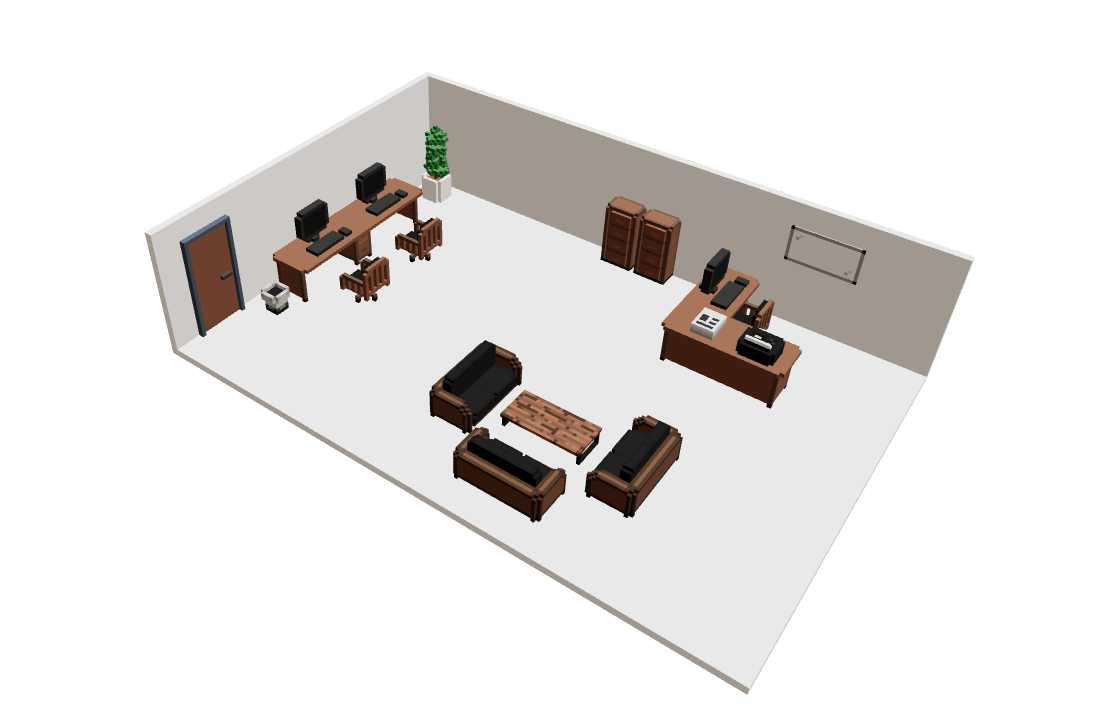
\includegraphics[width=5cm, height=4cm]{office.png}
          \end{center}
    \item Home - Dave's home where he spends time learning and creating.
          \begin{center}
              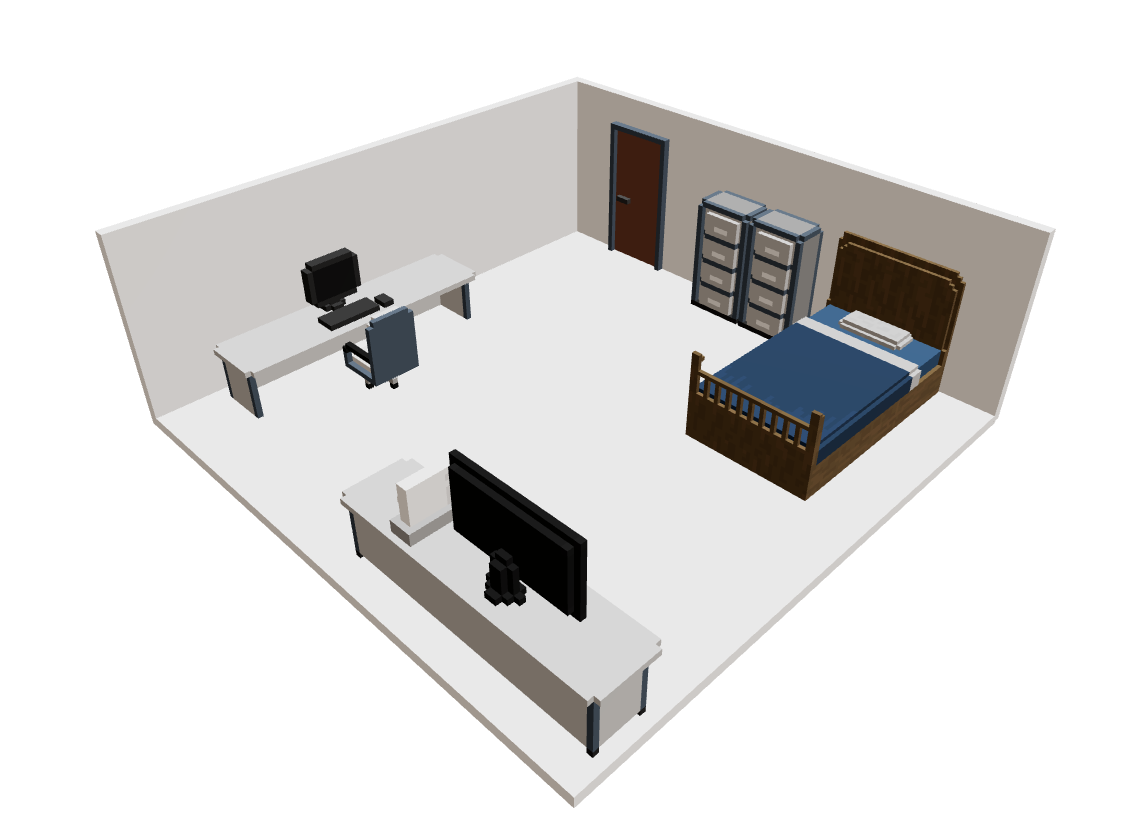
\includegraphics[width=5cm, height=4cm]{home.png}
          \end{center}
    \item Electronics shop - Dave buys circuit parts here from a salesman named Adem Shady
          \begin{center}
              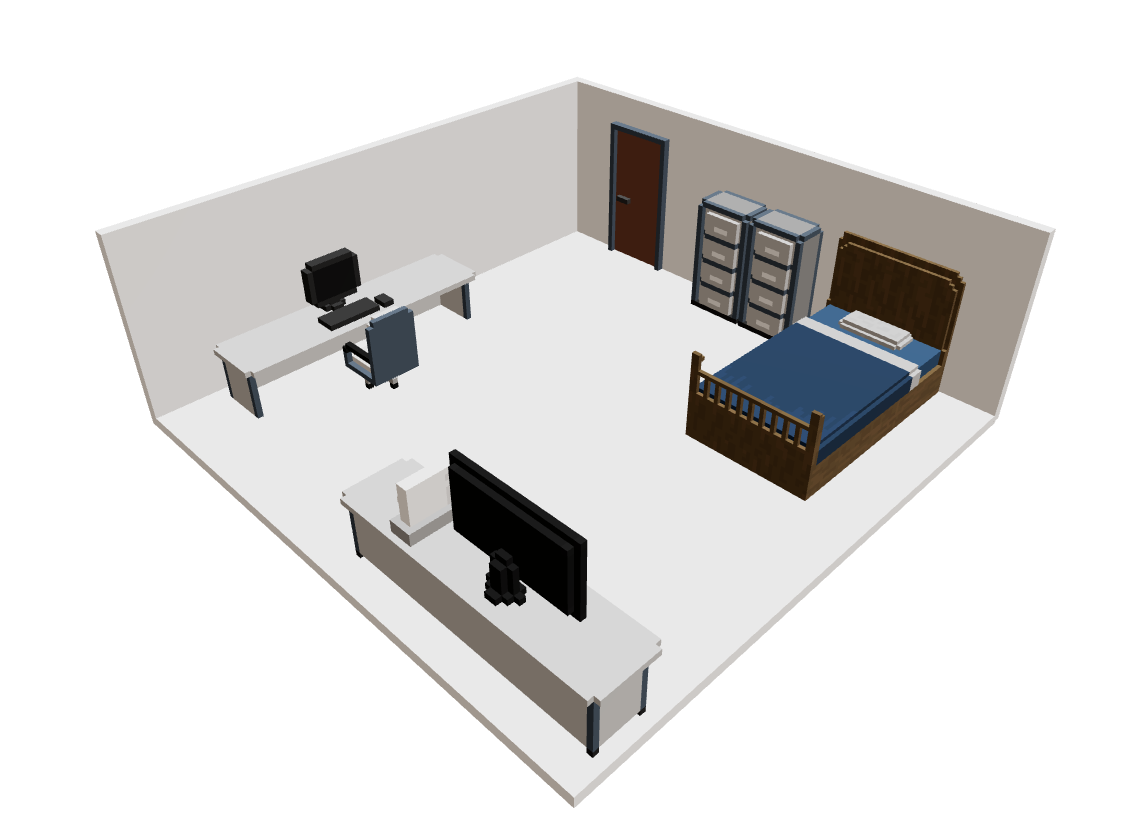
\includegraphics[width=5cm, height=4cm]{home.png}
          \end{center}
\end{enumerate}

Each of the mentioned 3D scenes will contain clickable elements that will open additional UI elements where the gameplay will actually happen 
like for example the circuit editor window.

\subsection{Gameplay}
The goal of the game is too build your own computer at home that can execute instructions of a predefined format (we made the instructions 
predefined so that we can validate the validity of the made computer by executing predefined programs).\\
The game will follow a linear path which is of the following form.\\
\begin{enumerate}
    \item Get an assignment from your boss 
    \item Solve the assignemt (this include producing various components and buying the necessary parts to make the components) 
    \item Get money for solving the assignment and unlock new components 
    \item Use those components to build other more complex components and systems at home 
    \item Once you progressed and unlocked every type of component you will get the final mission of building a computer  
    \item Once you build a computer that satisfies the given conditions (checked via tests made by the developers) you have officialy completed the main story of the game 
    \item After completing the game you unlock access to the black market where you can buy components made by other players and make anything you can imagine
\end{enumerate}







\section{Product market}
The audience for this product are electronics and computer enthusiasts aswell as college students.\\
THe product could be used by universities to teach computer architecture in a fun way engaging and rewarding way.\\
Profit will be earned by leveraging the game economy and reward ads. (Up to disscussion, detailed description needed).\\
\section{Product implementation}
The core simulator will be written in Rust (WASM) or in TS (ran in a seperate worker).

The frontend of this application will be made using the following technologies.\\
\begin{itemize}
    \item Svelte (Sveltekit) as the frontend framework
    \item Threlte (Three.js) as the webGL framework (library)
    \item TailwindCSS for styling
    \item Google adsense ads
\end{itemize}
The backend of this application will be made using the following technologies.\\
\begin{itemize}
    \item Vert.x as the backend web framework (toolkit more precisely)
    \item Postgres as the database
\end{itemize}
The application will be hosted on a VPS (most likely oracle on an oracle free VPS)
\end{document}